
%----------------------------------------------------------------------------------------
%	PACKAGES AND DOCUMENT CONFIGURATIONS BY DANIEL HEDIGER
%----------------------------------------------------------------------------------------

\documentclass{article}

\usepackage[version=3]{mhchem} % Package for chemical equation typesetting
\usepackage{siunitx} % Provides the \SI{}{} and \si{} command for typesetting SI units
\usepackage{graphicx} % Required for the inclusion of images
\usepackage{natbib} % Required to change bibliography style to APA
\usepackage{amsmath} % Required for some math elements 
\usepackage{german}
\usepackage{float}
\restylefloat{figure}
\usepackage[utf8]{inputenc}
\setlength\parindent{0pt} % Removes all indentation from paragraphs
\renewcommand{\labelenumi}{\alph{enumi}.} % Make numbering in the enumerate environment by letter rather than number (e.g. section 6)

%\usepackage{times} % Uncomment to use the Times New Roman font

%----------------------------------------------------------------------------------------
%	DOCUMENT INFORMATION
%----------------------------------------------------------------------------------------

\title{Physiklabor \\ Laborbericht \\ Wärme} % Title

\author{Daniel \textsc{Hediger} \\ Lucien \textsc{Egloff}} % Author name



\date{\today} % Date for the report

\begin{document}

\maketitle % Insert the title, author and date

\begin{center}
\begin{tabular}{l r}
Ausführungsdatum: & September 12, 2016 \\ % Date the experiment was performed
Dozent: & Dr.Ackermann % Instructor/supervisor
\end{tabular}
\end{center}
\newpage
\tableofcontents 

%----------------------------------------------------------------------------------------
%	SECTION 1
%----------------------------------------------------------------------------------------
\newpage
\section{Aufgabe 1}
Die spezifische Wärmekapazität einer Pfanne soll experimentell bestimmt werden.
\subsection{Grundlagen}
Die Wärmekapazität gibt an wie viel Energie benötigt wird um ein Kilogramm eines Materials um 1 Kelvin zu erhöhen.
Bei homogenen Körpern lässt sich die Wärmekapazität als Produkt der Masse des Körpers und der spezifischen Wärmekapazität berechnen.
\subsection{Versuchsaufbau}
\subsection{Resultate}
In dem idealisiert Versuch wird davon ausgegangen das keinen Wärmeaustausch über die Luft stattfindet.Um die Wärmekapazität der Pfanne zu bestimmen wurde die Mischtemperatur berechnet sowie auch gemessen. Da in diesem System die Energieerhaltung gilt, muss die Energiedifferenz die benötigte Energie sein um die Pfanne zu erwärmen.

Unter der Bedingung, dass keine Aggregatzustandsänderung auftritt und das System aus den Körpern abgeschlossen ist gilt:

\begin{equation}
\begin{split}
 Q_{abgegeben} = Q_{aufgenommen}\hspace{0.655cm}\\
 m_1\cdot c_1\cdot (T_1-T_m)=m_2\cdot c_2\cdot (T_2-T_m)
\end{split}
\end{equation}
Die aufgelöste Formel nach der Mischungstemperatur:
\begin{equation}
	T_m = \frac{m_1\cdot c_1\cdot T_1+m_2\cdot c_2\cdot T_2}{m_1\cdot c_1+m_2\cdot c_2}
\end{equation}
Aus der Mischtemperatur$(T_{mberechnet})$ und Mischtemperatur$(T_{mgemessen})$ kann die Wärme $Q$ berechnet werden, welche in die Pfanne übergegangen ist.
\begin{equation}
 Q = (m_{w1}+m_{w2}) \cdot c_w \cdot (T_m{berechnet}-T_m{gemessen})
\end{equation}
Somit kann die spezifische Wärmekapazität berechnet werden mit :
\begin{equation}
	c_{Pfanne} = \frac{Q}{m_{Pfanne} \cdot (T_{p1}-T_{p2}) }
\end{equation}

\textbf{Gegebene Grössen}

\textbf{Beschreibung Tabelle}

  \begin{description}
    \item[\textbf{ $Tw_k$}]= Temperatur des kalten Wasser in $[C^\circ]$
    \item[\textbf{ $Tw_w$}]= Temperatur des warmen Wasser in $[C^\circ]$
    \item[\textbf{ $mw_k$}]= Masse des kalten Wasser in $[g]$
    \item[\textbf{ $mw_w$}]= Masse des warmen Wasser in $[g]$
    \item[\textbf{ $Tm_g$}]= Gemessene Temperatur des Mischwasser in  $[C^\circ]$
    \item[\textbf{ $Tm_g$}]= Berechnete Temperatur des Mischwasser in  $[C^\circ]$
    \item[\textbf{ $c$}]=  Berechnete spez. Wärmekapazität  $[\frac{Kg}{J \cdot K}]$
    
  \end{description}
\begin{table}[h]
    \begin{tabular}{|l|l|l|l|l|l|l|l|}
    
        \hline
        Durchgang &\textbf{$Tw_k$} &\textbf{$Tw_w$}& \textbf{$mw_k$}&\textbf{$mw_w$}&\textbf{$Tm_g$}&\textbf{$Tm_b$}&\textbf{$c$}\\ \hline
        1         & 18.6 & 55 & 645& 276 & 31.8 &29.5&1329.34\\ 
        2         & 18.2 & 63 &500 &240  & 44 &32.73&1329.34\\ 
        3         & 16 & 69 &659 &497  &41 &36.73&805.43\\ 
        4         &  18.2  &50 & 780 & 709 &33&33.74&305.02\\ \hline
        \textbf{Mittel} &\textbf{17.75}&\textbf{59.25}&\textbf{646}  &\textbf{430.5}  &\textbf{37.45} &\textbf{33.18}&\textbf{} \\ 
        \hline
    \end{tabular}
\end{table}

\subsection*{Schlussfolgerung}

\section{Versuch 2}
Bestimmen Sie die spezifische Schmelzwärme von Eis indem Sie Eis in die mit Wasser gefüllte Pfanne geben.
Halten Sie die Wassertemperatur als Funktion der Zeit in einem Diagramm fest. Führen Sie das Experiment
mit einem grossen Eisklotz und mit zerdrücktem Eis durch.
\subsection{Grundlage}
Bei diesem Versuch wurde bei einer bestimmten Menge Wasser und bestimmter Anfangstemperatur 
Eis dazugegeben. Es gilt die Temperaturänderung des Wassers in Funktion der Zeit aufzuzeigen. 
Dabei gilt es eine angemessene Anfangstemperatur des Wassers festzulegen um sicherzustellen, dass 
der Schmelzversuch nicht zu langsam aber auch nicht zu schnell von statten geht. Doch vorerst 
mussten folgende Messwerte ermittelt werden
\subsection{Versuchsaufbau}
\subsection{Resultate}
\subsection{Schlussfolgerung}
Gemäss Tabelle aus dem Taschenbuch der Physik von Horst Kuchling S.636 beträgt der Wert der 
Schmelzwärme von Eis 334kJ/kg.  
Da es sich bei diesem Versuch um Zerdrücktes Eis und dieses eine viel grössere Fläche gegenüber 
dem Wasser ergibt, beträgt hier die Schmelzwärme einiges weniger. Da bei diesem Experiment die 
Versuchszeit ziemlich kurz war, wurde die Wärmekapazität der Pfanne ignoriert, da sich diese über 
diese kurze Dauer nicht gross veränderte. 
\section{Versuch 3}
\subsection{Grundlage}
\subsection{Versuchsaufbau}
\begin{figure}[H]
\begin{center}


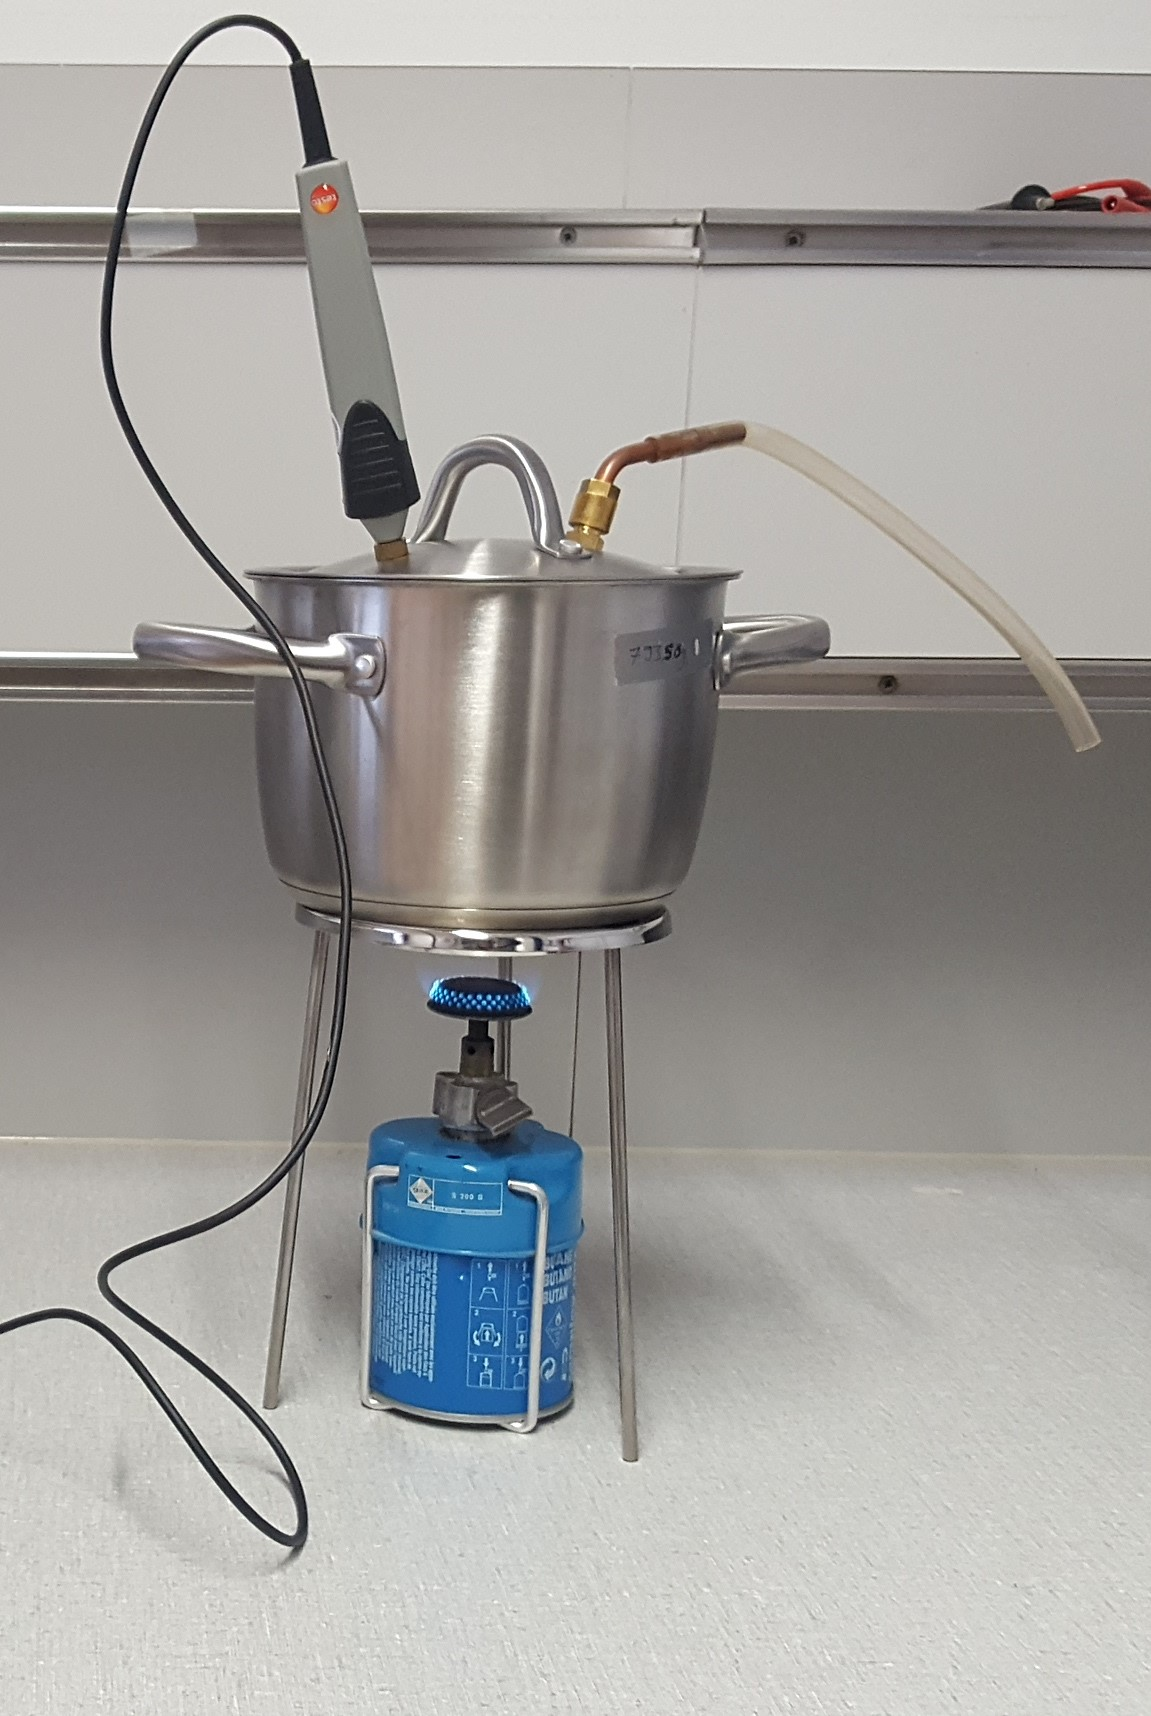
\includegraphics[scale=0.3]{Waerme1.pdf} 
\caption{Wasser wird über dem Gaskocher erhitzt.}
\end{center}
\end{figure}
\subsection{Resultate}
\begin{figure}[H]
\includegraphics[scale=0.5]{Waerme.pdf} 
\caption{Gemessene Grössen und Trendverlauf.}
\end{figure}
\subsection{Schlussfolgerung}
\section{Versuch 4}
Die spezifische Verdampfungs‐ bez. Kondensationswärme soll bestimmt werden, indem der Wasserdampf in eine
mit Wasser gefüllte Pfanne geführt wird.
\subsection{Grundlage}
Bei diesem Versuch soll eine gewisse Menge Wasser in einem Isolierten Kochtopf mittels der 
Dampfwärme aus einem anderen Kochtopf erwärmt werden. Der Kochtopf und das zu erwärmende 
Wasser im Isoliertopf sind über ein kleines Röhrensystem miteinander verbunden. Dabei soll der 
Temperaturverlauf des zu erwärmenden Wassers sowie die Gewichtsveränderung gemessen werden. 
\subsection{Versuchsaufbau}
\begin{figure}[H]
\includegraphics[scale=0.5]{Pot.pdf} 
\caption{Durch verdampfen und wider kondensieren soll Energie von dem rechten in den linken Topf gelangen.}
\end{figure}
\subsection{Resultate}

\subsection{Schlussfolgerung}
\end{document}